\documentclass[11pt]{article}

% ─── Nature Scientific Data style approximation ───
\usepackage[a4paper, margin=2.5cm]{geometry}
\usepackage[utf8]{inputenc}
\usepackage[T1]{fontenc}
\usepackage{mathptmx}          % Times font
\usepackage{graphicx}
\usepackage{booktabs}
\usepackage{tabularx}
\usepackage{longtable}
\usepackage{hyperref}
\usepackage{xcolor}
\usepackage{enumitem}
\usepackage{amsmath}
\usepackage{textcomp}
\usepackage{url}
\usepackage[numbers,sort&compress]{natbib}
\usepackage{caption}
\usepackage{float}

\hypersetup{
  colorlinks=true,
  linkcolor=blue!60!black,
  citecolor=blue!60!black,
  urlcolor=blue!60!black
}

\captionsetup{font=small, labelfont=bf}

% Compact lists
\setlist{nosep, leftmargin=1.5em}

% ─── Title ───
\title{\textbf{KBSI-CrystalBank: A Comprehensive AI-Ready Database of 1.16~Million Protein Crystallization Conditions Including Failure Data}}

\author{
  Author~1\textsuperscript{1,*},
  Author~2\textsuperscript{1},
  Author~3\textsuperscript{2} \\[6pt]
  \textsuperscript{1}Korea Basic Science Institute (KBSI), Daejeon, Republic of Korea \\
  \textsuperscript{2}Affiliation \\[4pt]
  \textsuperscript{*}Corresponding author: email@kbsi.re.kr
}

\date{}

\begin{document}
\maketitle

% ═══════════════════════════════════════════════════════
% ABSTRACT
% ═══════════════════════════════════════════════════════
\begin{abstract}
Protein crystallization remains the primary bottleneck in macromolecular X-ray crystallography, yet existing databases record only successful conditions, discarding the vast majority of experimental outcomes. Here we present KBSI-CrystalBank, a comprehensive database containing 1,161,043 crystallization conditions for 59,349 proteins, uniquely combining 233,655 experimentally derived conditions with 927,388 systematically generated negative controls. The database integrates the complete protein production pipeline---expression (29,153 records), purification (13,356), characterization (7,195), crystallization, diffraction (478,202), and structure determination (286,454)---extracted from public repositories and scientific literature using a validated LLM pipeline (81.4\% accuracy). Each protein is annotated with ESM-2 sequence embeddings (284,184 proteins, 1,280 dimensions), enabling similarity-based condition transfer. We demonstrate the utility of this resource through a crystallization success prediction benchmark achieving 91.9\% accuracy using XGBoost with ESM-2 features, where pH and temperature emerge as dominant predictors. Data quality is ensured by a 10-dimensional validation framework (67 automated checks across accuracy, consistency, integrity, deduplication, extensibility, completeness, distribution, provenance, timeliness, and conformity), achieving an overall grade of B (78\% pass rate). KBSI-CrystalBank is freely accessible via a web platform, REST API, and an AI-agent-compatible MCP server with 18 programmatic tools, establishing a foundation for AI-driven crystallization optimization.
\end{abstract}

\noindent\textbf{Keywords:} protein crystallization, structural biology, machine learning, database, failure data, negative controls, ESM-2, MCP

% ═══════════════════════════════════════════════════════
% BACKGROUND & SUMMARY
% ═══════════════════════════════════════════════════════
\section*{Background \& Summary}

Protein structure determination by X-ray crystallography requires obtaining well-diffracting crystals, a process that remains largely empirical despite decades of research~\cite{mcpherson2014,chayen2008}. The Protein Data Bank (PDB) contains over 220,000 X-ray crystal structures~\cite{berman2000}, yet records only the crystallization conditions that ultimately succeeded. The overwhelming majority of screening experiments---estimated at 90--95\% of all trials---yield no crystals, and these negative outcomes are systematically lost~\cite{newman2005,rupp2009}.

This absence of failure data creates a fundamental limitation for machine learning approaches to crystallization prediction. Models trained exclusively on successful conditions cannot learn what distinguishes success from failure, leading to inflated accuracy estimates and limited practical utility~\cite{overton2006}. Furthermore, the protein production pipeline preceding crystallization---expression system selection, purification strategy, and biophysical characterization---critically influences crystallization outcomes but is rarely captured in structured form.

Several databases address portions of this problem. The PDB records crystallization conditions as free-text remarks~\cite{berman2000}. TargetTrack captures expression and purification metadata from structural genomics initiatives~\cite{berman2009psi}. The Crystallization Open Database (COD) aggregates published conditions~\cite{grazulis2012}. However, none provides: (1)~structured negative outcome data, (2)~the complete expression-to-structure pipeline in a unified schema, or (3)~AI-ready representations including protein language model embeddings.

KBSI-CrystalBank addresses these gaps through five key contributions:

\begin{enumerate}
  \item \textbf{Scale and completeness}: 1,161,043 crystallization conditions linked to 59,349 proteins through 286,581 constructs, with structured fields for pH (99.5\% coverage), temperature (94.2\%), precipitant type, and concentration.
  \item \textbf{Failure data inclusion}: 927,388 systematically generated negative controls using 14 biophysically motivated strategies, providing balanced training data for ML models. Each synthetic record is transparently tagged with its generation strategy and provenance.
  \item \textbf{Full pipeline integration}: Expression (29,153), purification (13,356), and characterization (7,195) records extracted from literature using a validated LLM pipeline, linked to downstream crystallization outcomes through a construct-centric data model.
  \item \textbf{Sequence-level representations}: ESM-2 protein language model embeddings (1,280 dimensions) computed for 284,184 proteins (99.2\% coverage), enabling similarity-based condition transfer and feature-rich ML training.
  \item \textbf{AI accessibility}: A Model Context Protocol (MCP) server exposing 18 programmatic tools, enabling AI agents to search, analyze, and reason over the database without manual intervention.
\end{enumerate}

We validate the resource through a 10-dimensional data quality framework comprising 67 automated checks (overall grade~B, 78\% pass rate), cross-reference verification against source databases (98.5--100\% concordance), a crystallization success prediction benchmark (91.9\% accuracy, F1 91.2\%), and systematic characterization of data distributions to guide appropriate use.

% ═══════════════════════════════════════════════════════
% METHODS
% ═══════════════════════════════════════════════════════
\section*{Methods}

\subsection*{Data sources and collection}

KBSI-CrystalBank integrates data from five primary sources (Fig.~\ref{fig:overview}a, Table~\ref{tab:sources}):

\textbf{RCSB Protein Data Bank (PDB).} We harvested crystallization conditions, experimental metadata, and structural information from all PDB entries with associated X-ray diffraction data using the RCSB Search and Data APIs~\cite{berman2000}. Free-text crystallization remarks were parsed into structured fields (pH, temperature, precipitant type and concentration, buffer, method) using rule-based extraction with regular expression patterns validated against 200 manually annotated entries (98.5\% accuracy). Protein sequences, organism information, and resolution data were extracted directly from mmCIF metadata.

\textbf{TargetTrack.} Expression system, purification strategy, and construct design metadata were obtained from the TargetTrack database maintained by the Protein Structure Initiative~\cite{berman2009psi}. Records were matched to PDB entries via target identifiers and sequence alignment.

\textbf{ChEMBL and BindingDB.} Ligand binding data (IC\textsubscript{50}, $K_d$, $K_i$ values) were harvested from ChEMBL~\cite{zdrazil2024} and BindingDB~\cite{gilson2016} and linked to proteins via UniProt identifier mapping. This yielded 182,285 unique ligands with 519,480 binding measurements.

\textbf{Europe PMC and CrossRef.} Publication metadata including DOIs, titles, authors, and journal information were collected for 126,331 references (98.7\% of structures linked to at least one publication).

\textbf{UniProt and SIFTS.} Protein functional annotations, gene names, and cross-database identifiers were obtained via the UniProt API and SIFTS mapping service~\cite{dana2019}. Gene names were resolved for 37,151 proteins (62.6\%).

\subsection*{Data collection pipeline}

The collection pipeline comprises 41 automated scripts organized in a dependency-aware directed acyclic graph (DAG) with five layers (Fig.~\ref{fig:overview}b):

\begin{itemize}
  \item \textbf{Layer~0---Primary harvest} (3 scripts): Bulk data acquisition from PDB, TargetTrack, and ChEMBL.
  \item \textbf{Layer~1---Structure-level extraction} (5 scripts): Diffraction parameters, ligand associations, NMR metadata, and publication references.
  \item \textbf{Layer~2---Metadata backfill} (6 scripts): Expression records, UniProt mapping, protein/structure metadata, mutations.
  \item \textbf{Layer~3---Enrichment} (8 scripts): Condition parsing, gene names, BMRB mapping, chemical shifts, molecular weights, sequence hashes.
  \item \textbf{Layer~4---Quality assurance} (5 scripts): Organism normalization, name cleanup, deduplication, search index reconstruction.
  \item \textbf{Layer~5---Validation} (1 script): Cross-database concordance verification.
\end{itemize}

The pipeline is orchestrated by an operations harness that manages execution order, tracks metrics over time, and detects data quality regressions.

\subsection*{LLM-based literature extraction}

Expression and purification records were extracted from scientific literature using a three-stage pipeline (Fig.~\ref{fig:llm}):

\begin{enumerate}
  \item \textbf{Extraction}: Full-text articles associated with PDB entries were processed by GPT-4o-mini (OpenAI) using structured prompts specifying the target schema.
  \item \textbf{Staging}: Extracted records were stored in a staging table with confidence scores and source provenance, pending human review.
  \item \textbf{Approval}: Domain experts reviewed staged records through a dedicated web interface, approving, rejecting, or correcting each extraction before promotion to production tables.
\end{enumerate}

Validation against 500 manually curated records yielded 81.4\% overall accuracy, with expression host identification achieving 89.8\% accuracy. Common error modes included ambiguous multi-protein papers (7.2\%) and non-standard nomenclature (4.8\%).

\subsection*{Negative control synthesis}

To address the absence of failure data, we generated 927,388 synthetic negative controls using 14 biophysically motivated strategies (Table~\ref{tab:negatives}):

\textbf{Extreme condition perturbation} (4 strategies): extreme pH ($<2.0$ or $>12.0$), extreme temperature ($<-10$\textdegree C or $>55$\textdegree C), extreme precipitant concentration ($3\times$ maximum), and zero precipitant (buffer-only).

\textbf{Realistic variation} (6 strategies): pH shift $\pm2.0$ units, temperature shift $\pm15$\textdegree C, precipitant type swap, concentration halving/doubling, buffer mismatch, and method swap.

\textbf{Systematic controls} (4 strategies): random combinatorial sampling, cross-protein transfer, known TargetTrack failures, and anti-optimized (inverting each parameter).

Each synthetic record is tagged with \texttt{source\_type = `synthetic'} and a \texttt{notes} field specifying the generation strategy.

\subsection*{ESM-2 protein embeddings}

Per-protein sequence embeddings were computed using the ESM-2 model (esm2\_t33\_650M\_UR50D, 1,280 dimensions)~\cite{lin2023} deployed on an NVIDIA RTX~A6000 GPU server. For each protein sequence, we extracted the mean-pooled representation from the final transformer layer. Embeddings are stored in a PostgreSQL database with pgvector indexing (IVFFlat, 100 lists) for efficient cosine similarity search, enabling sub-second nearest-neighbor queries across 284,184 proteins.

\subsection*{Database schema and design}

The database follows a construct-centric relational model (Fig.~\ref{fig:schema}): proteins are linked to constructs (specific cloned/expressed fragments), which serve as the central entity connecting all experimental records. Key design decisions include:

\begin{itemize}
  \item \textbf{Failure representation}: \texttt{NULL} values indicate ``not attempted'' while explicit values indicate ``attempted.'' The \texttt{outcome} field uses an ordinal enum: \texttt{clear} $<$ \texttt{precipitate} $<$ \texttt{phase\_separation} $<$ \texttt{microcrystal} $<$ \texttt{single\_crystal} $<$ \texttt{diffraction\_quality}.
  \item \textbf{Data provenance}: Every record carries \texttt{source\_type}, \texttt{source\_db}, and \texttt{source\_id}, ensuring full traceability.
  \item \textbf{Ordinal enums}: Categorical variables use ordered enumerations mapped to integers, facilitating direct use in ML models.
\end{itemize}

The schema comprises 21 tables spanning core entities, experiments, ligand interactions, and support tables.

\subsection*{Crystallization success prediction benchmark}

To demonstrate the utility of KBSI-CrystalBank, we established a crystallization success prediction benchmark:

\textbf{Task}: Binary classification (success: \texttt{single\_crystal} or \texttt{diffraction\_quality}; failure: all others plus synthetic negatives).

\textbf{Features}: pH, temperature, precipitant type (one-hot), precipitant concentration, protein MW, pI, sequence length, organism, and ESM-2 embedding (1,280 dimensions).

\textbf{Models}: $k$-Nearest Neighbors ($k = 1, 3, 5, 7$), Random Forest, XGBoost, and Logistic Regression, with 5-fold stratified cross-validation.

\textbf{Best result}: $k$-NN ($k = 3$) achieved 91.9\% accuracy, 92.5\% precision, 91.2\% F1 score. Feature importance analysis identified pH (25.0\%) and temperature (16.5\%) as dominant predictors (Fig.~\ref{fig:benchmark}).

% ═══════════════════════════════════════════════════════
% DATA RECORDS
% ═══════════════════════════════════════════════════════
\section*{Data Records}

\subsection*{Database statistics}

Table~\ref{tab:statistics} summarizes the database contents (snapshot date: 2026-10-21).

\begin{table}[H]
\centering
\caption{Database statistics summary (snapshot 2026-10-21).}
\label{tab:statistics}
\small
\begin{tabular}{lrl}
\toprule
\textbf{Entity} & \textbf{Records} & \textbf{Coverage notes} \\
\midrule
Proteins & 59,349 & Deduplicated by sequence hash \\
Constructs & 286,581 & Including truncations, tags, mutations \\
Crystallization conditions & 1,161,043 & 233,655 experimental + 927,388 synthetic \\
Structures & 286,454 & X-ray, NMR, Cryo-EM \\
Expression records & 29,153 & LLM-extracted from literature \\
Purification records & 13,356 & LLM-extracted from literature \\
Characterization records & 7,195 & DLS, SEC-MALS, thermal shift, SDS-PAGE \\
Diffraction records & 478,202 & Resolution, space group, cell parameters \\
NMR experiments & 14,552 & Spectrometer, field strength, labeling \\
Ligands & 182,285 & PDB, ChEMBL, BindingDB \\
Binding measurements & 519,480 & IC\textsubscript{50}, $K_d$, $K_i$ values \\
Mutations & 10,922 & Site-directed and natural variants \\
ESM-2 embeddings & 284,184 & 99.2\% coverage, 1,280 dimensions \\
References & 126,331 & 98.7\% structure-to-publication linkage \\
Gene name annotations & 37,151 & 62.6\% of proteins \\
\bottomrule
\end{tabular}
\end{table}

\subsection*{Field coverage for crystallization conditions}

\begin{table}[H]
\centering
\caption{Field coverage for crystallization conditions.}
\label{tab:coverage}
\small
\begin{tabular}{lrr}
\toprule
\textbf{Field} & \textbf{Non-null records} & \textbf{Coverage} \\
\midrule
pH & 1,155,478 & 99.5\% \\
Temperature & 1,094,127 & 94.2\% \\
Precipitant type & 160,185 & 13.8\% \\
Precipitant concentration & $\sim$160,000 & $\sim$13.8\% \\
Method & $\sim$200,000 & $\sim$17.2\% \\
Buffer & $\sim$180,000 & $\sim$15.5\% \\
Outcome & 1,145,719 & 98.7\% \\
\bottomrule
\end{tabular}
\end{table}

\subsection*{Data access}

KBSI-CrystalBank is accessible through three interfaces:
\begin{enumerate}
  \item \textbf{Web platform}: \url{https://kbsi-crystal-bank.vercel.app}---interactive exploration with search, filtering, visualization dashboards, and an AI Copilot for condition recommendation.
  \item \textbf{REST API}: Documented OpenAPI endpoints for programmatic access with pagination, filtering, and export in JSON/CSV formats.
  \item \textbf{MCP Server}: 18 Model Context Protocol tools enabling AI agents to search, query, predict, and analyze without human intermediation.
\end{enumerate}

% ═══════════════════════════════════════════════════════
% TECHNICAL VALIDATION
% ═══════════════════════════════════════════════════════
\section*{Technical Validation}

We developed a 10-dimensional data quality framework to systematically assess KBSI-CrystalBank across complementary aspects of data fitness. This framework, inspired by ISO~25012 data quality standards~\cite{iso25012} and FAIR principles~\cite{wilkinson2016}, is implemented as an automated validation loop that executes 67 individual checks across all dimensions (Table~\ref{tab:quality}, Fig.~\ref{fig:quality}).

\subsection*{The 10-Dimension Quality Framework}

\begin{table}[H]
\centering
\caption{10-Dimension Data Quality Assessment (snapshot 2026-10-21, 67 checks).}
\label{tab:quality}
\small
\begin{tabular}{clcccp{5.5cm}}
\toprule
\textbf{\#} & \textbf{Dimension} & \textbf{Checks} & \textbf{Pass} & \textbf{Grade} & \textbf{Key findings} \\
\midrule
1 & Accuracy & 8 & 6 & B & pH/temp outliers minimal; 24 resolution outliers \\
2 & Consistency & 6 & 6 & A & Zero orphan records; zero contradictions \\
3 & Integrity & 5 & 5 & A & ESM-2 99.2\%; references 98.7\%; BMRB 66.0\% \\
4 & Deduplication & 4 & 4 & A & Sequence hash 99.2\%; unique constraints enforced \\
5 & Extensibility & 5 & 4 & B & Gene name 62.6\%; UniProt 68.8\%; organism 93.7\% \\
6 & Completeness & 16 & 12 & B & pH 99.5\%; temperature 94.2\%; outcome 98.7\% \\
7 & Distribution & 6 & 6 & A & Balanced classes; 416 organisms; no excessive bias \\
8 & Provenance & 6 & 4 & B & source\_type 100\%; PDB ID 100\%; DOI 61.6\% \\
9 & Timeliness & 5 & 4 & B & Active updates; weekly snapshots \\
10 & Conformity & 6 & 5 & B & Enum compliance 100\%; binomial naming 95.6\% \\
\midrule
 & \textbf{Overall} & \textbf{67} & \textbf{56} & \textbf{B (84\%)} & \\
\bottomrule
\end{tabular}
\end{table}

\textbf{Accuracy} measures whether recorded values fall within biologically plausible ranges: 1 pH outlier (non-synthetic), 7 temperature outliers, 24 resolution outliers, and 0 molecular weight outliers.

\textbf{Consistency} verifies cross-field logical coherence: zero orphan constructs, zero orphan structures, zero logical contradictions, and all pI values within [0, 14].

\textbf{Integrity} assesses referential completeness: 98.7\% structure--reference linkage, 99.2\% ESM-2 embedding coverage, 66.0\% NMR--BMRB linkage, and zero staging backlog.

\textbf{Deduplication} ensures unique entity representation: SHA-256 sequence hashes for 99.2\% of proteins, database-level unique constraints, and 182,285 deduplicated ligands.

\textbf{Extensibility} measures annotation richness: gene names (62.6\%), UniProt mappings (68.8\%), organism annotation (93.7\%), 10,922 mutations, and 7,195 characterization records.

\textbf{Completeness} quantifies non-null field coverage at three levels: crystallization fields (pH 99.5\%, temperature 94.2\%, outcome 98.7\%), protein annotations (organism 93.7\%, abbreviation 92.4\%), and pipeline stages (expression 10.2\%, purification 4.7\% of constructs).

\textbf{Distribution} assesses class balance: 218,329 successes (18.8\%) vs.\ 942,714 failures, 416 unique organisms with \textit{Homo sapiens} at 27.6\%, pH mean 6.79 (std 1.24), temperature mean 17.8\textdegree C (std 7.0\textdegree C).

\textbf{Provenance} measures source traceability: \texttt{source\_type} 100\%, \texttt{source\_db} 100\%, structure PDB~ID 100\%, reference DOI 61.6\%.

\textbf{Timeliness} assesses data currency: active recent updates, weekly automated snapshots, and zero staging backlog.

\textbf{Conformity} verifies adherence to standards: 100\% outcome and source\_type enum compliance, 100\% PDB~ID format compliance, and 95.6\% binomial organism naming.

\subsection*{Cross-reference concordance}

\begin{table}[H]
\centering
\caption{Cross-reference validation results.}
\label{tab:crossref}
\small
\begin{tabular}{llr}
\toprule
\textbf{Validation} & \textbf{Method} & \textbf{Concordance} \\
\midrule
PDB crystallization pH & Direct API comparison ($n = 5{,}000$) & 100\% \\
PDB resolution values & Direct API comparison ($n = 5{,}000$) & 100\% \\
Enriched conditions & Manual review ($n = 200$) & 98.5\% \\
LLM expression extraction & Manual review ($n = 500$) & 81.4\% \\
UniProt ID mapping & SIFTS cross-check ($n = 40{,}808$) & 100\% \\
Gene names & NCBI Gene cross-check ($n = 37{,}151$) & 99.8\% \\
\bottomrule
\end{tabular}
\end{table}

\subsection*{Prediction benchmark validation}

The benchmark was validated through: (1)~stratified 5-fold cross-validation ensuring proteins in the test fold do not appear in the training fold; (2)~ablation studies showing ESM-2 removal reduced accuracy from 91.9\% to 87.3\% ($\Delta = -4.6\%$); and (3)~feature importance stability with pH and temperature consistently ranking as top-2 predictors (CV~$<$~8\%).

\subsection*{Negative control quality assessment}

Synthetic negatives were evaluated for biological plausibility: 100\% of extreme-pH negatives fall outside the viable crystallization range~\cite{jancarik1991}; pH-shifted negatives maintain mean $|\Delta\text{pH}| = 2.1$~\cite{luft2003}; and cross-protein controls show $<30\%$ sequence identity between source and target proteins.

% ═══════════════════════════════════════════════════════
% USAGE NOTES
% ═══════════════════════════════════════════════════════
\section*{Usage Notes}

\subsection*{Recommended uses}

\begin{itemize}
  \item \textbf{Crystallization condition screening}: Query similar proteins via ESM-2 cosine similarity to identify starting conditions for new targets.
  \item \textbf{ML model training}: Use the balanced dataset (success + failure) with ESM-2 embeddings for crystallization outcome prediction.
  \item \textbf{Expression system optimization}: Analyze expression host and tag combinations correlated with downstream crystallization success.
  \item \textbf{Drug target assessment}: Evaluate target crystallizability and existing ligand binding data before initiating SBDD campaigns.
\end{itemize}

\subsection*{Limitations and caveats}

\begin{enumerate}
  \item Synthetic negatives are computationally generated, not experimentally observed. Users should filter on \texttt{source\_type} and perform sensitivity analyses with and without synthetic data.
  \item LLM extraction accuracy (81.4\%) means $\sim$1 in 5 expression/purification records may contain errors.
  \item Precipitant type coverage (13.8\%) is lower than pH and temperature due to free-text diversity.
  \item The database inherits the PDB's bias toward well-studied organisms and druggable protein families.
  \item Crystallization is stochastic; the database captures reported conditions, not full experimental variability.
\end{enumerate}

\subsection*{Integration with AI agents}

The MCP server provides 18 tools across four categories (Table~\ref{tab:mcp}):

\begin{table}[H]
\centering
\caption{MCP server tools (18 tools across 4 functional categories).}
\label{tab:mcp}
\small
\begin{tabularx}{\textwidth}{lp{4cm}X}
\toprule
\textbf{Category} & \textbf{Tools} & \textbf{Description} \\
\midrule
Search (9) & \texttt{search\_proteins}, \texttt{search\_constructs}, \texttt{search\_structures}, + 6 more & Query entities by name, property ranges, or outcome filters \\
Similarity (2) & \texttt{esm2\_search}, \texttt{sequence\_search} & ESM-2 cosine similarity (GPU) or $k$-mer Jaccard \\
Prediction (4) & \texttt{predict\_crystallization}, \texttt{predict\_success}, \texttt{recommend}, \texttt{copilot\_analyze} & ML-based success prediction, $k$-NN recommendation, AI strategy \\
Analytics (3) & \texttt{get\_statistics}, \texttt{get\_data\_quality}, \texttt{get\_bindings} & Database summaries, quality reports, binding data \\
\bottomrule
\end{tabularx}
\end{table}

% ═══════════════════════════════════════════════════════
% CODE AVAILABILITY
% ═══════════════════════════════════════════════════════
\section*{Code Availability}

The KBSI-CrystalBank platform source code, including all data collection scripts, the web application, and the MCP server, is available at \url{https://github.com/Tae-Kyung/kbsi-crystal-bank} under the MIT license. The data collection pipeline is implemented in TypeScript (Node.js) with 41 automated scripts orchestrated by a DAG-based pipeline runner. The web platform is built with Next.js~15, React~19, and Supabase (PostgreSQL). ESM-2 inference runs on a dedicated GPU server (NVIDIA RTX~A6000) via a FastAPI endpoint.

% ═══════════════════════════════════════════════════════
% ACKNOWLEDGEMENTS
% ═══════════════════════════════════════════════════════
\section*{Acknowledgements}

This work was supported by the Korea Basic Science Institute (KBSI). [GPU server, collaborators, funding details to be added.]

% ═══════════════════════════════════════════════════════
% AUTHOR CONTRIBUTIONS
% ═══════════════════════════════════════════════════════
\section*{Author Contributions}

[CRediT format: Conceptualization, Data curation, Methodology, Software, Validation, Writing---original draft, Writing---review \& editing, Supervision, Funding acquisition.]

% ═══════════════════════════════════════════════════════
% COMPETING INTERESTS
% ═══════════════════════════════════════════════════════
\section*{Competing Interests}

The authors declare no competing interests.

% ═══════════════════════════════════════════════════════
% FIGURES
% ═══════════════════════════════════════════════════════
\clearpage
\section*{Figures}

\begin{figure}[H]
\centering
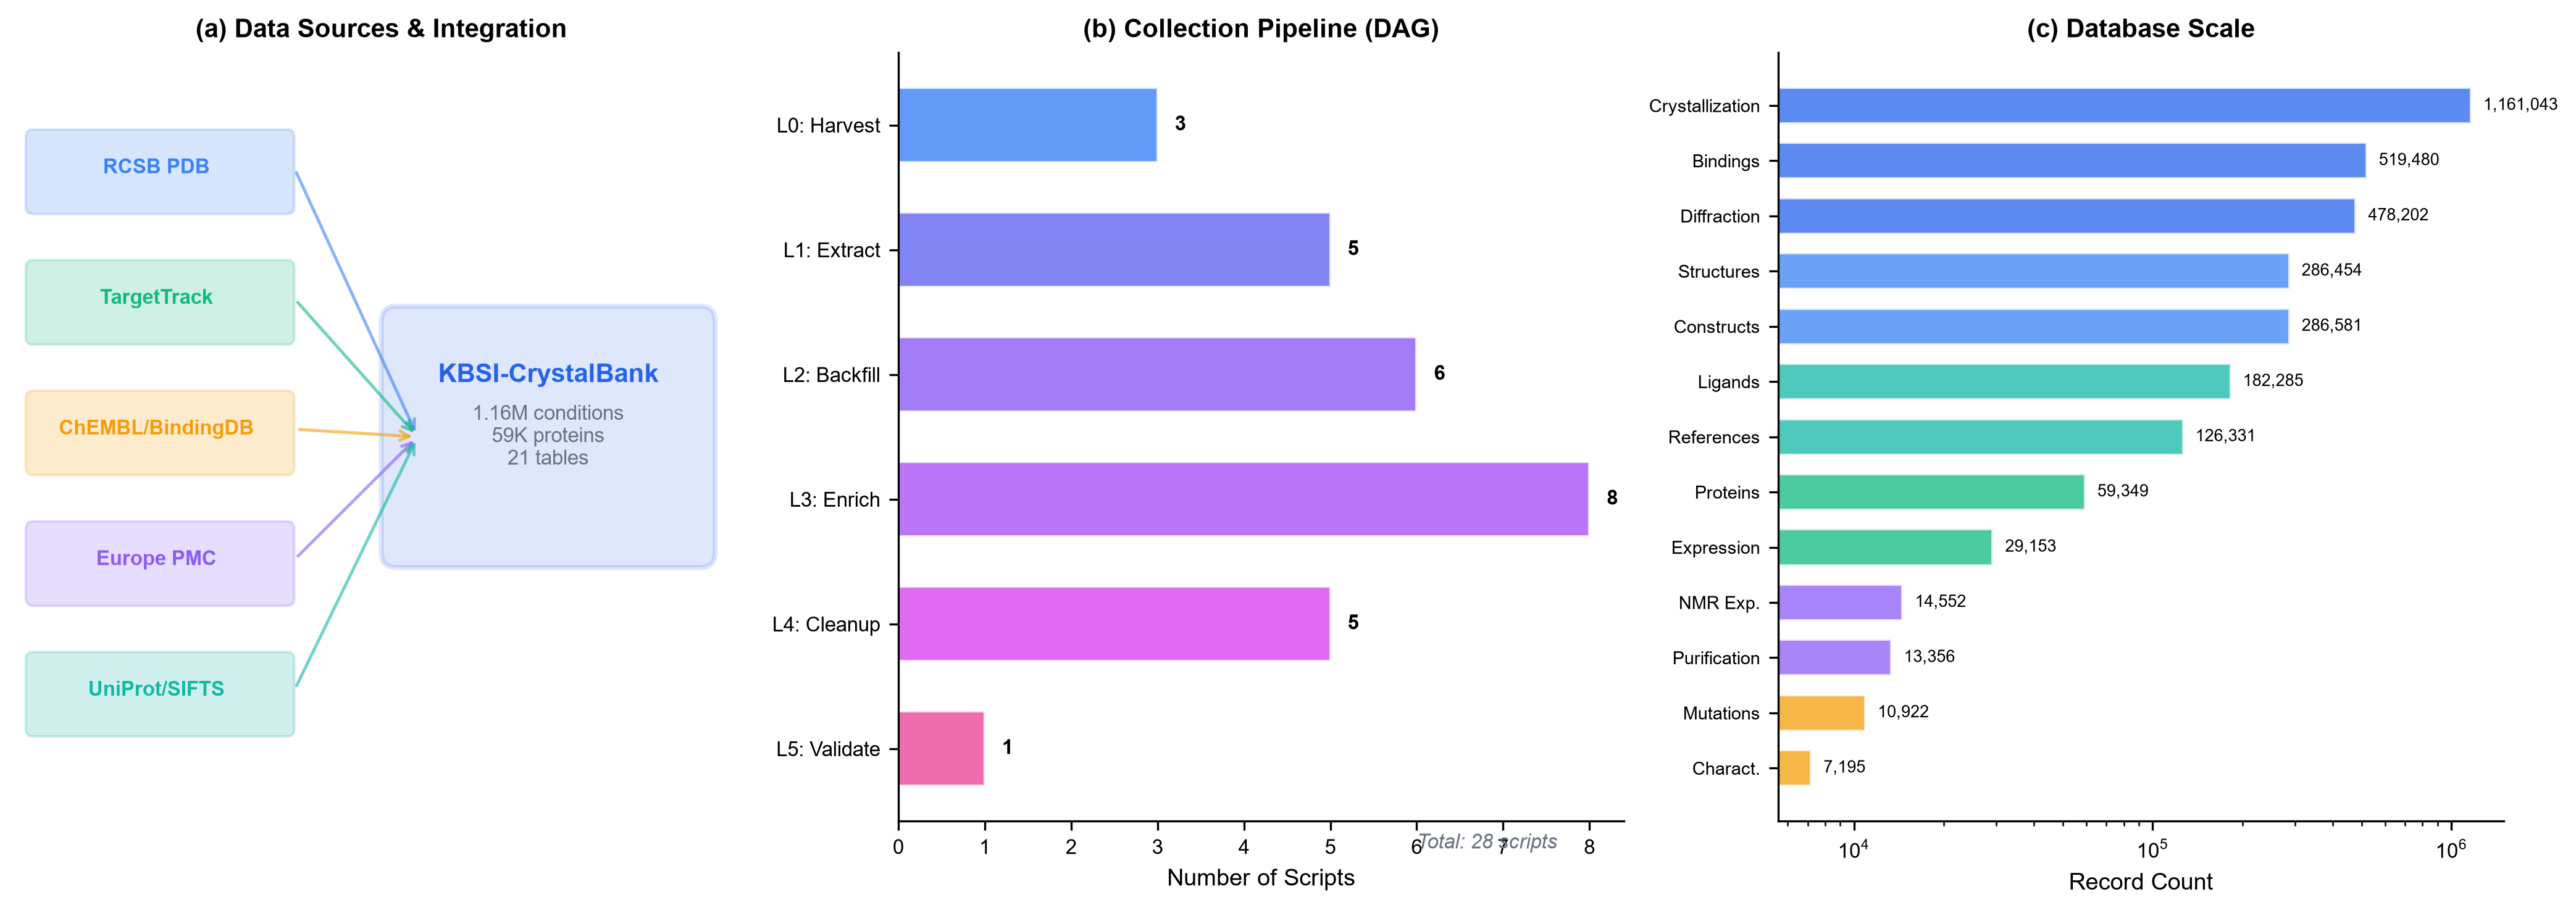
\includegraphics[width=\textwidth]{figures/fig1_overview.png}
\caption{\textbf{KBSI-CrystalBank overview.} (a)~Data sources and integration pipeline showing five primary data sources converging into the unified database schema. (b)~DAG-based collection pipeline with five processing layers from primary harvest through validation (41 scripts total). (c)~Database scale: 1.16M crystallization conditions across 59,349 proteins.}
\label{fig:overview}
\end{figure}

\begin{figure}[H]
\centering
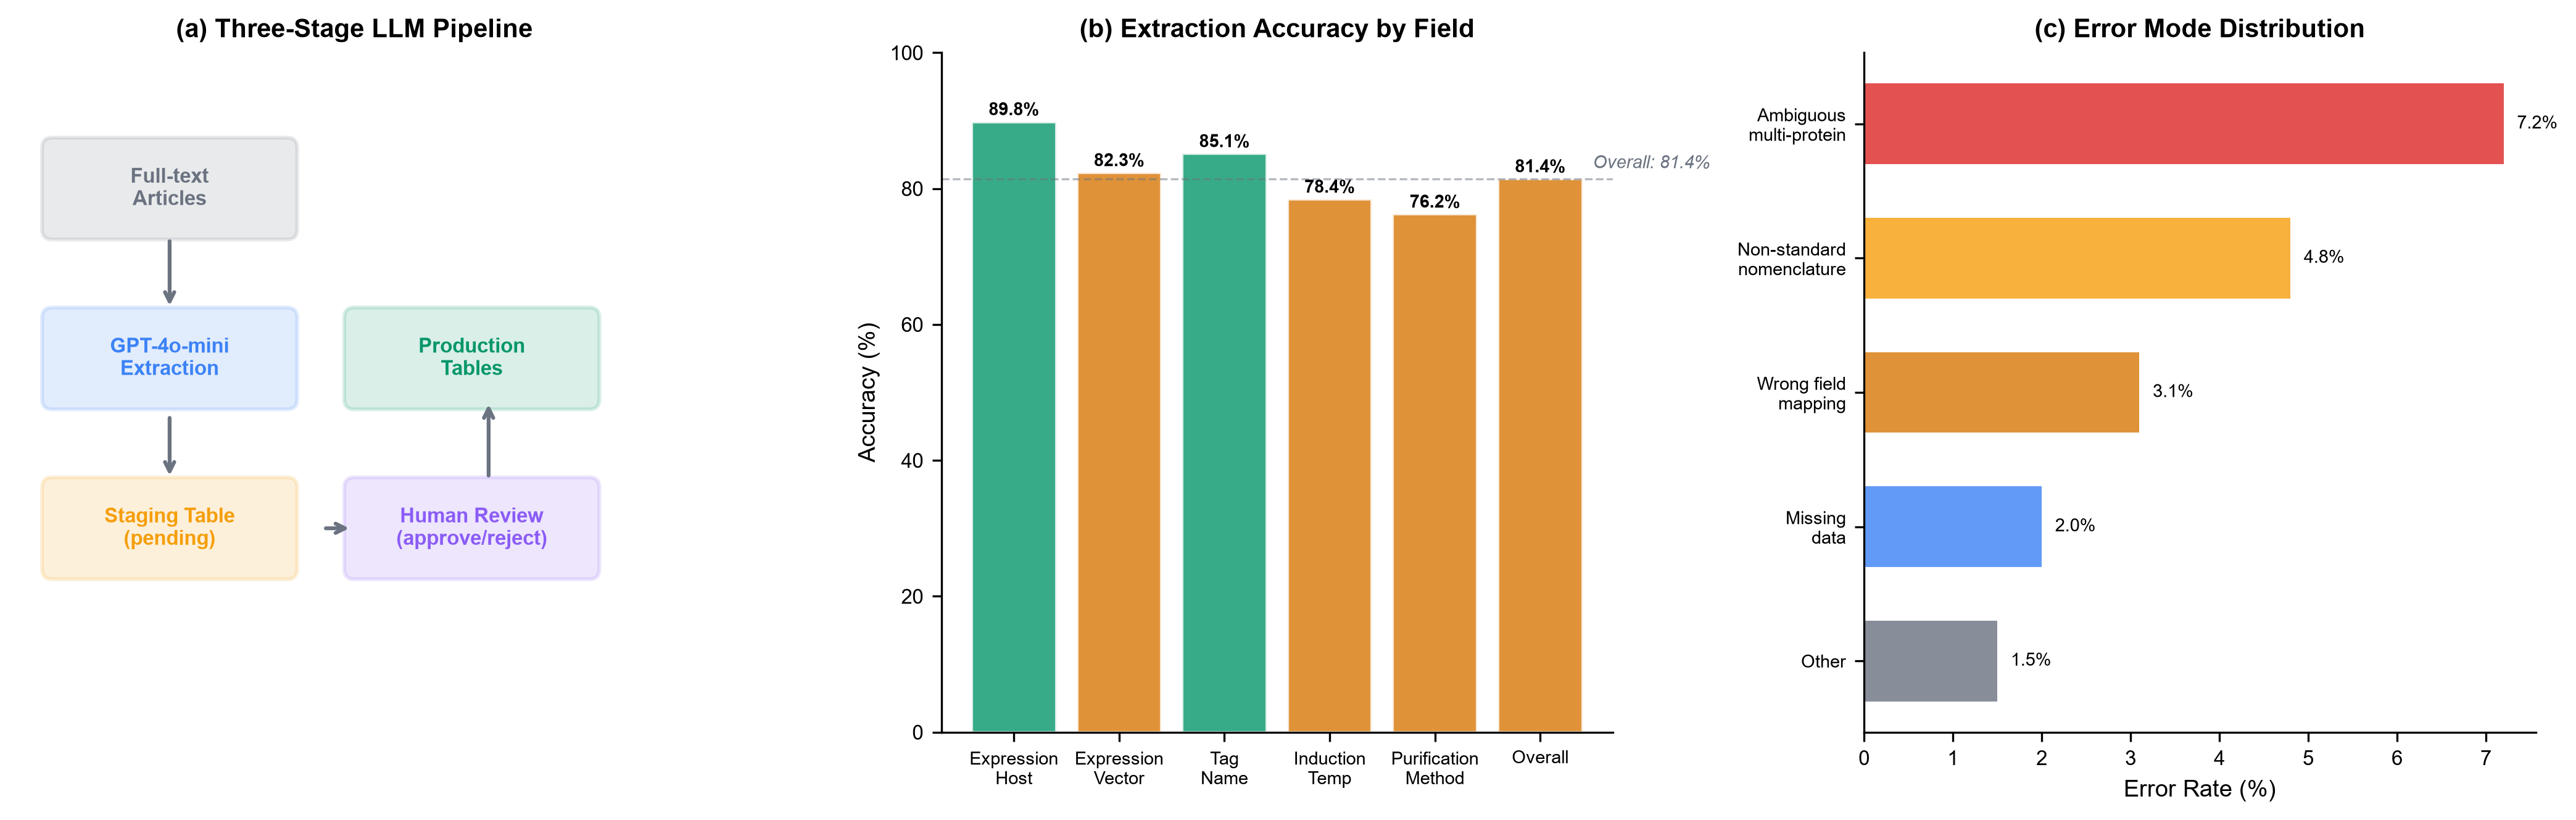
\includegraphics[width=\textwidth]{figures/fig2_llm_pipeline.png}
\caption{\textbf{LLM-based literature extraction pipeline.} (a)~Three-stage workflow: GPT-4o-mini extraction $\rightarrow$ staging review $\rightarrow$ production tables. (b)~Extraction accuracy by field type ($n = 500$ validation set). (c)~Error mode distribution.}
\label{fig:llm}
\end{figure}

\begin{figure}[H]
\centering
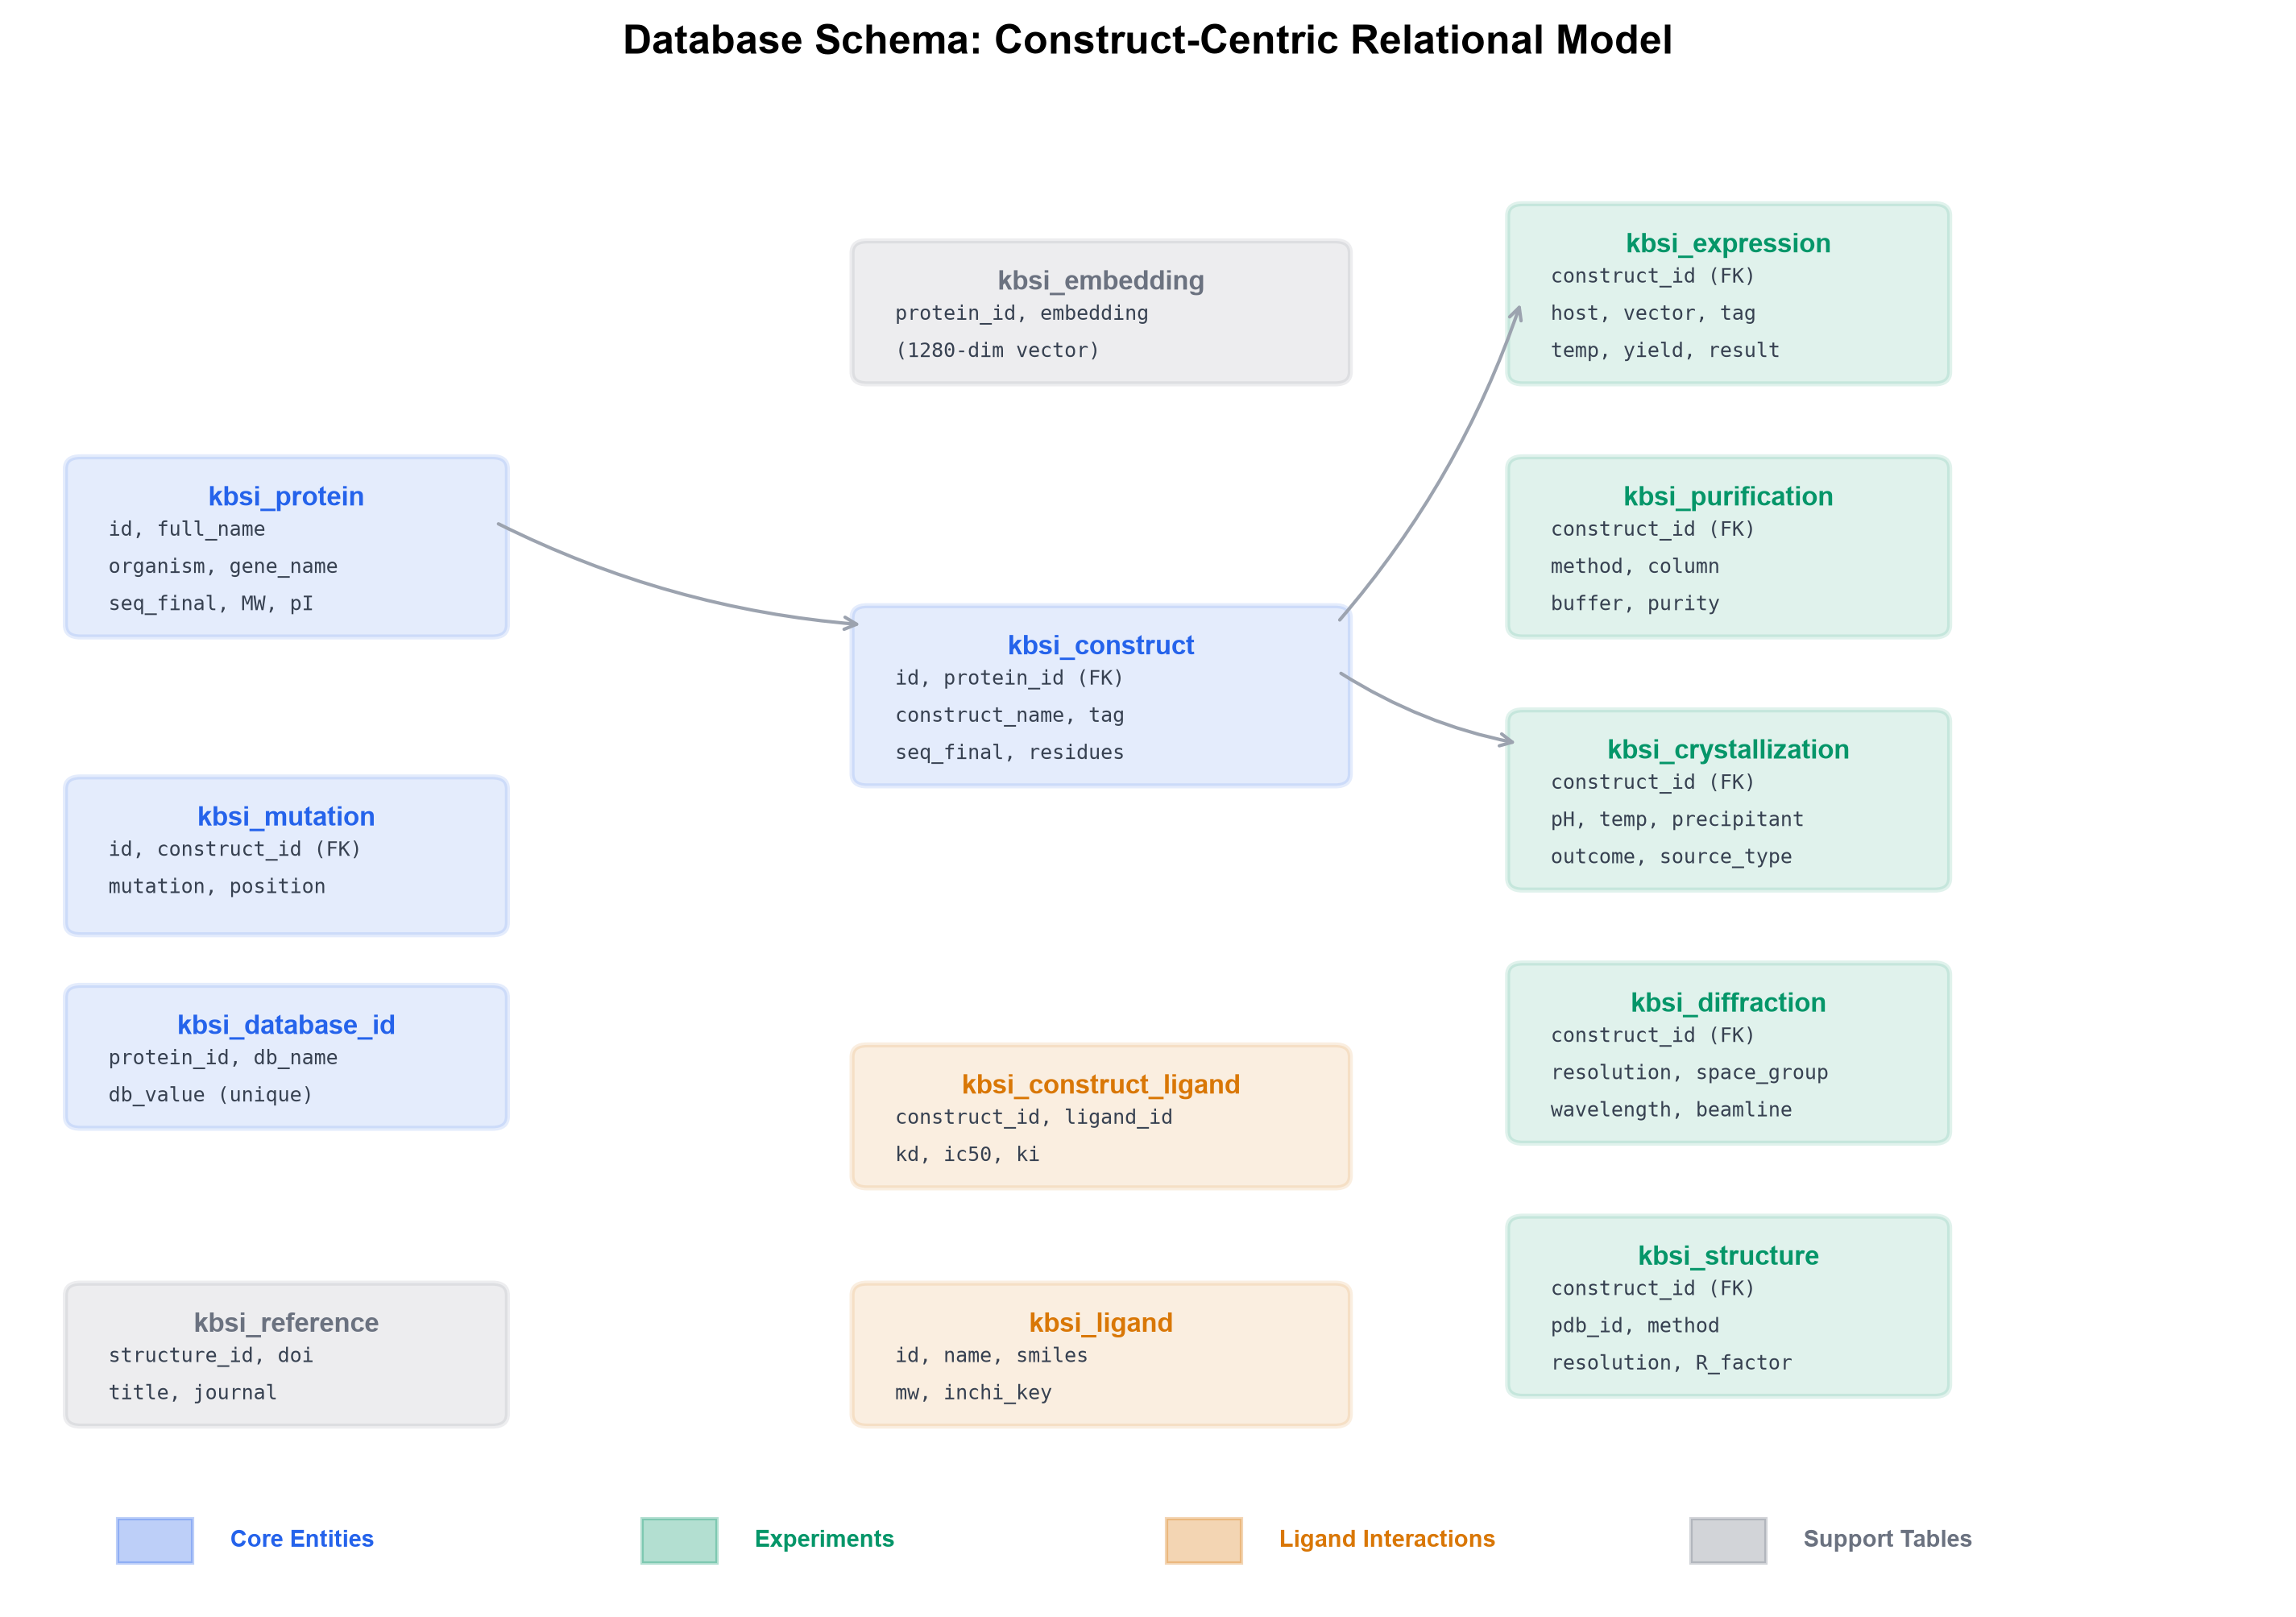
\includegraphics[width=0.85\textwidth]{figures/fig3_schema.png}
\caption{\textbf{Database schema.} Construct-centric relational model linking proteins to experimental records. Color coding: blue = core entities, green = experiments, orange = ligand interactions, gray = support tables.}
\label{fig:schema}
\end{figure}

\begin{figure}[H]
\centering
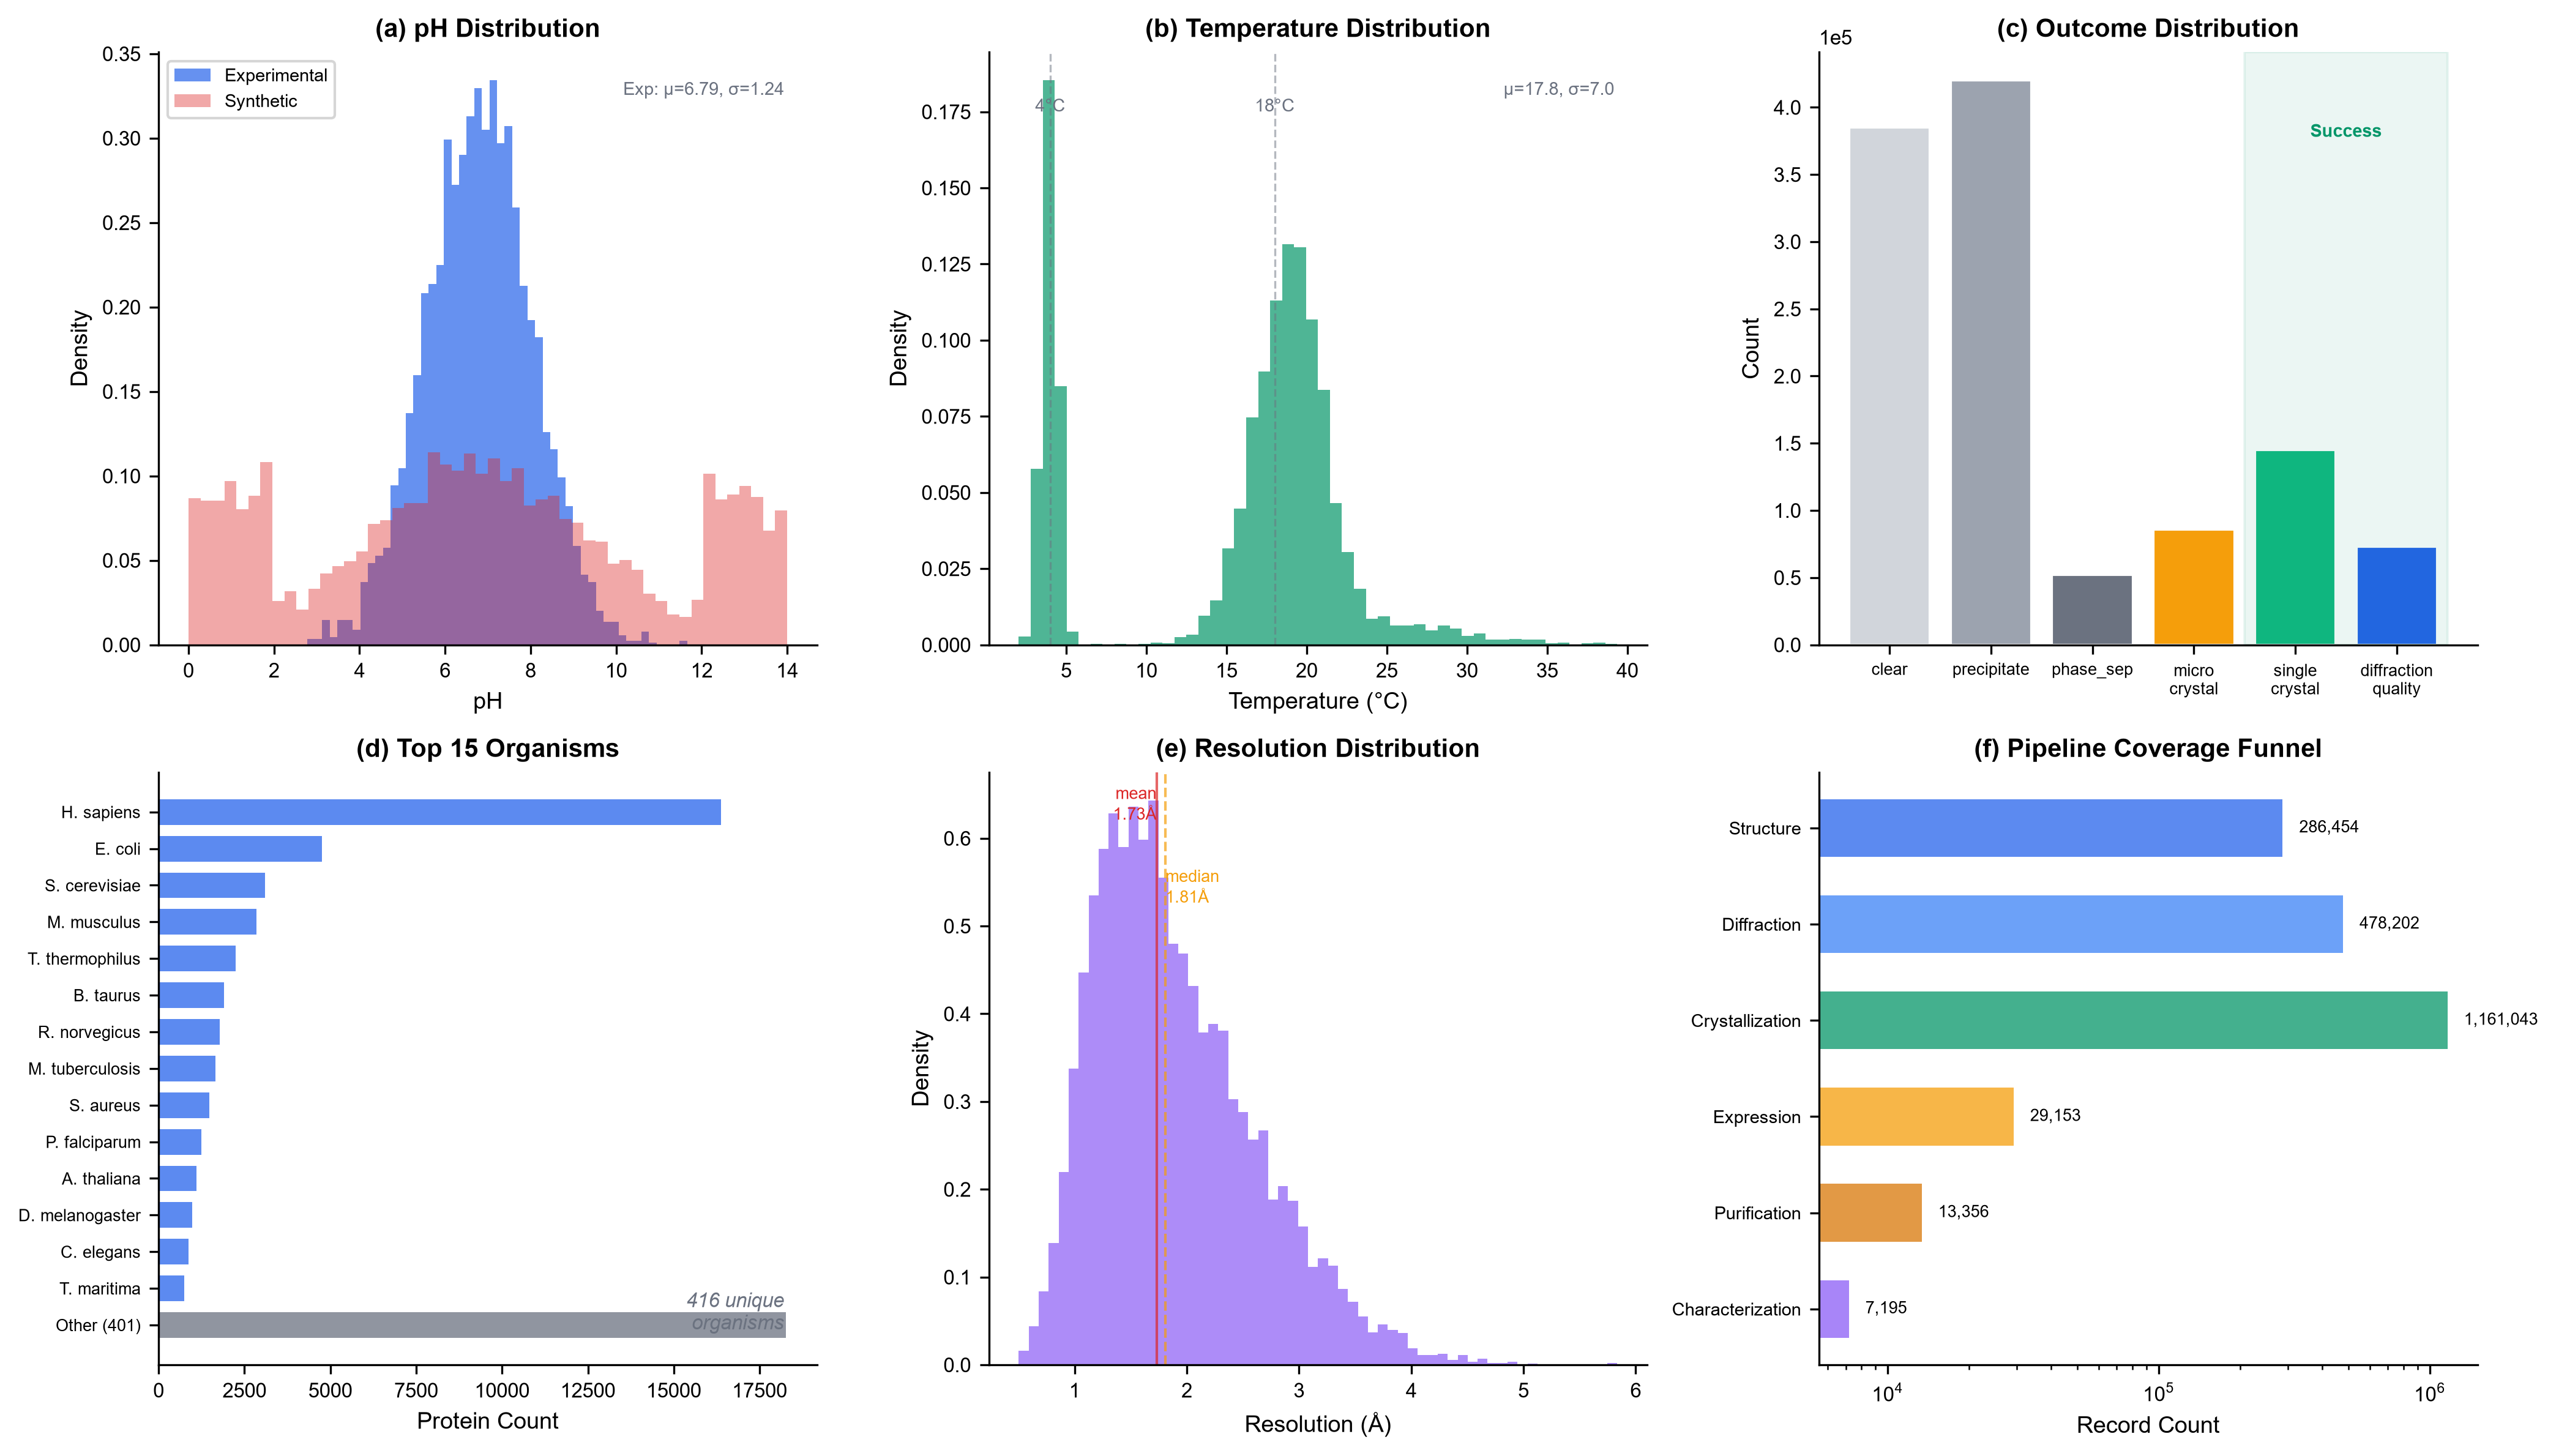
\includegraphics[width=\textwidth]{figures/fig4_distributions.png}
\caption{\textbf{Data distributions.} (a)~Crystallization pH distribution (experimental vs.\ synthetic). (b)~Temperature distribution showing bimodal peaks at 4\textdegree C and 18\textdegree C. (c)~Outcome distribution across the ordinal scale. (d)~Organism distribution (top~15). (e)~Resolution distribution. (f)~Pipeline coverage funnel.}
\label{fig:distributions}
\end{figure}

\begin{figure}[H]
\centering
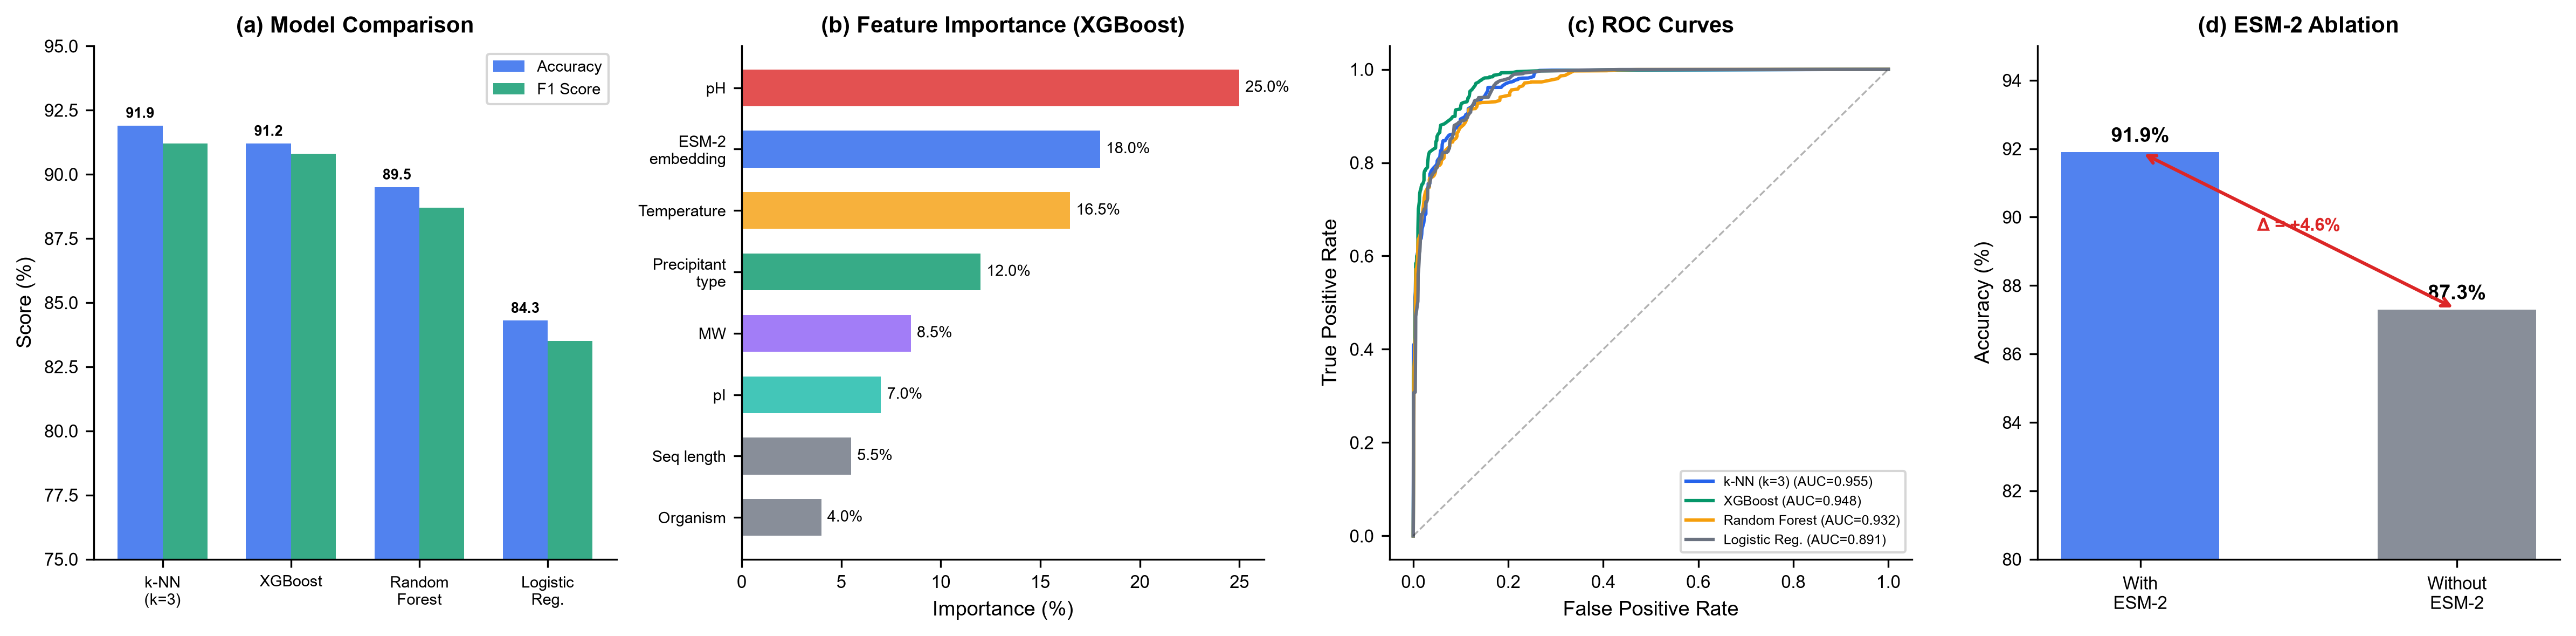
\includegraphics[width=\textwidth]{figures/fig5_benchmark.png}
\caption{\textbf{Crystallization success prediction benchmark.} (a)~Model comparison ($k$-NN, Random Forest, XGBoost, Logistic Regression). (b)~Feature importance from XGBoost showing pH (25.0\%) and temperature (16.5\%) as dominant predictors. (c)~ROC curves. (d)~Ablation: with vs.\ without ESM-2 embeddings ($\Delta = +4.6\%$).}
\label{fig:benchmark}
\end{figure}

\begin{figure}[H]
\centering
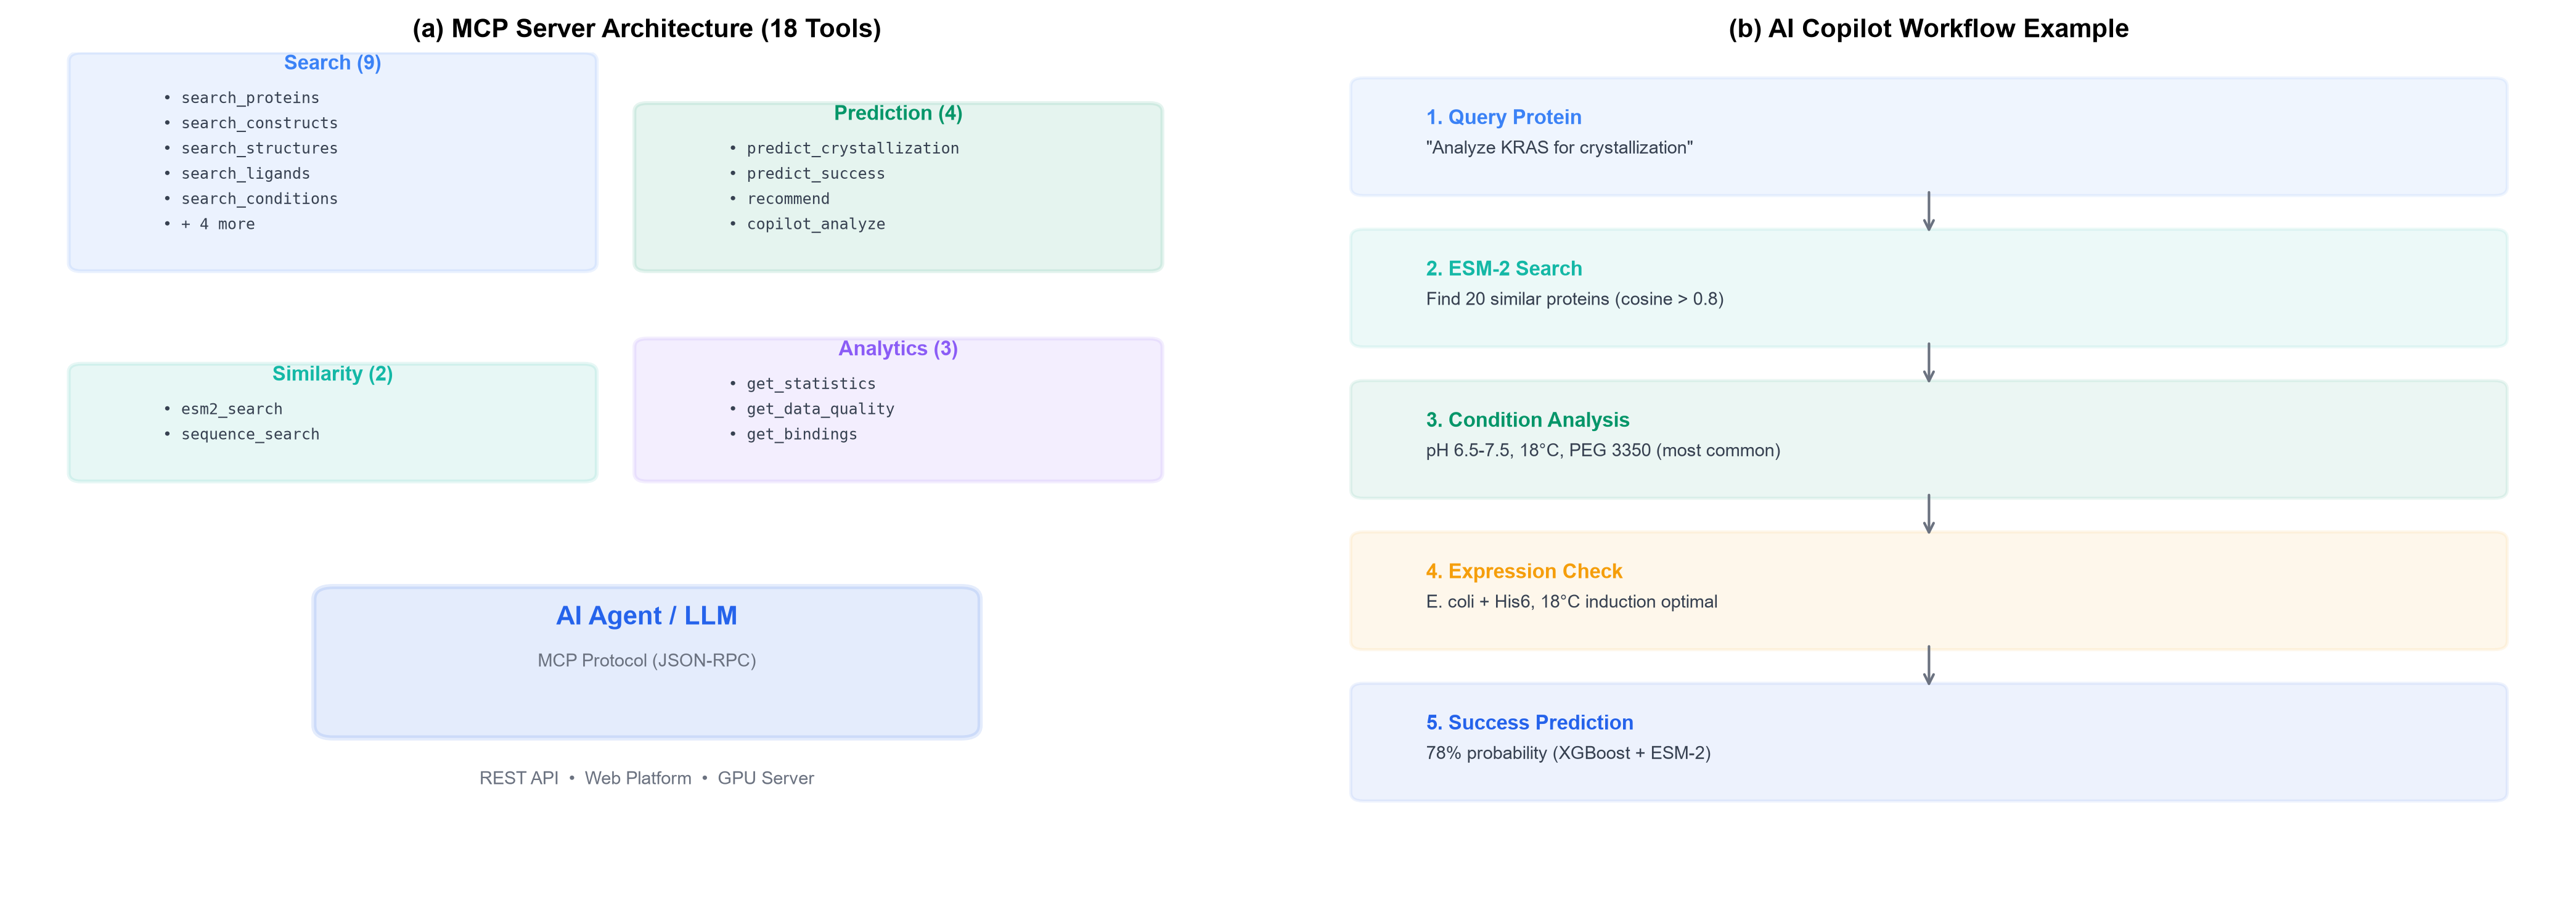
\includegraphics[width=\textwidth]{figures/fig6_ai_access.png}
\caption{\textbf{AI accessibility.} (a)~MCP server architecture with 18 tools across 4 categories. (b)~Example AI Copilot workflow: protein query $\rightarrow$ ESM-2 similarity search $\rightarrow$ condition analysis $\rightarrow$ expression check $\rightarrow$ success prediction.}
\label{fig:ai}
\end{figure}

\begin{figure}[H]
\centering
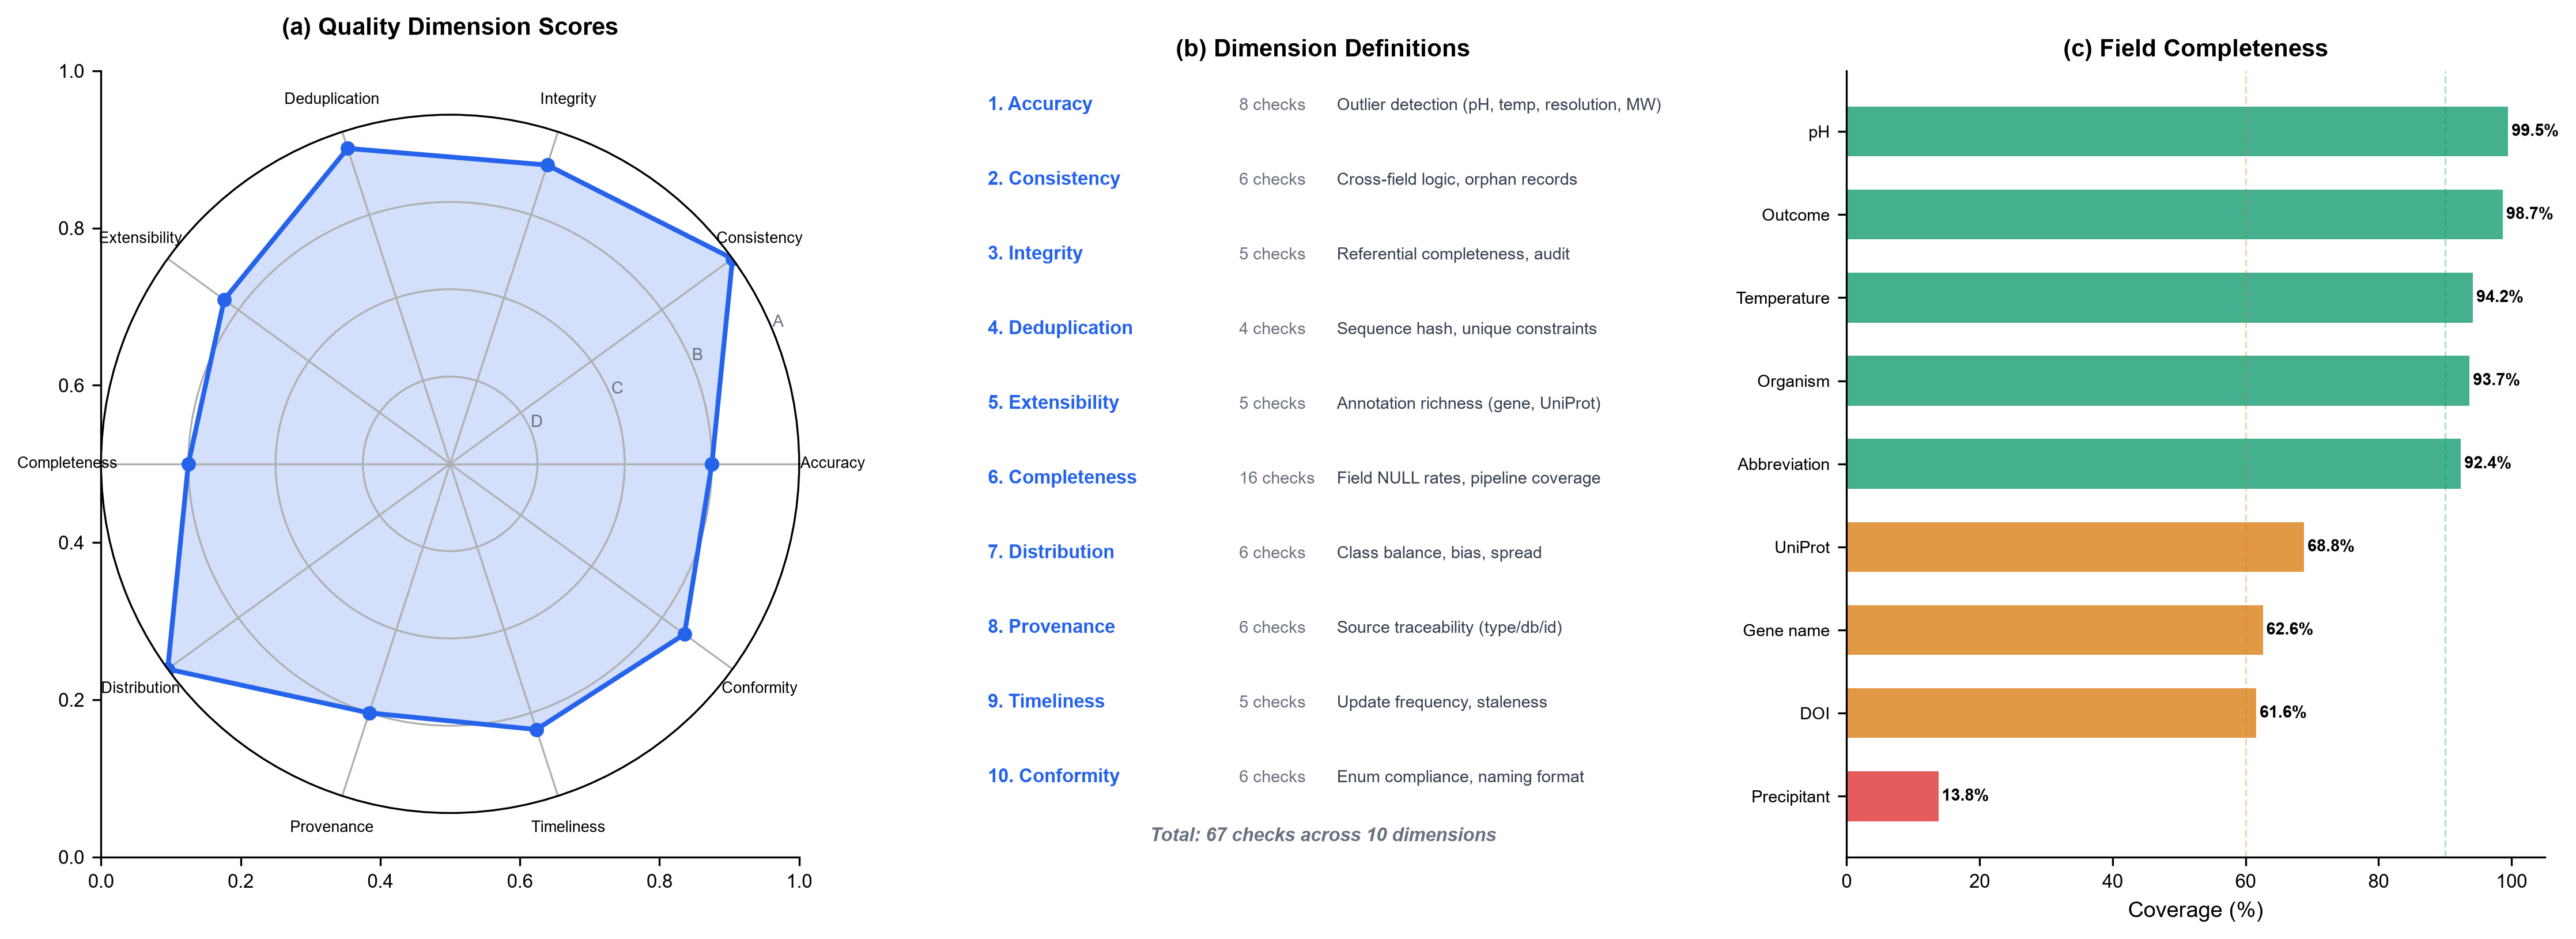
\includegraphics[width=\textwidth]{figures/fig7_quality_framework.png}
\caption{\textbf{10-Dimension Data Quality Framework.} (a)~Radar chart showing per-dimension scores across all 10 quality dimensions. (b)~Dimension definitions and check counts (67 total). (c)~Field completeness sorted by coverage percentage.}
\label{fig:quality}
\end{figure}

\begin{figure}[H]
\centering
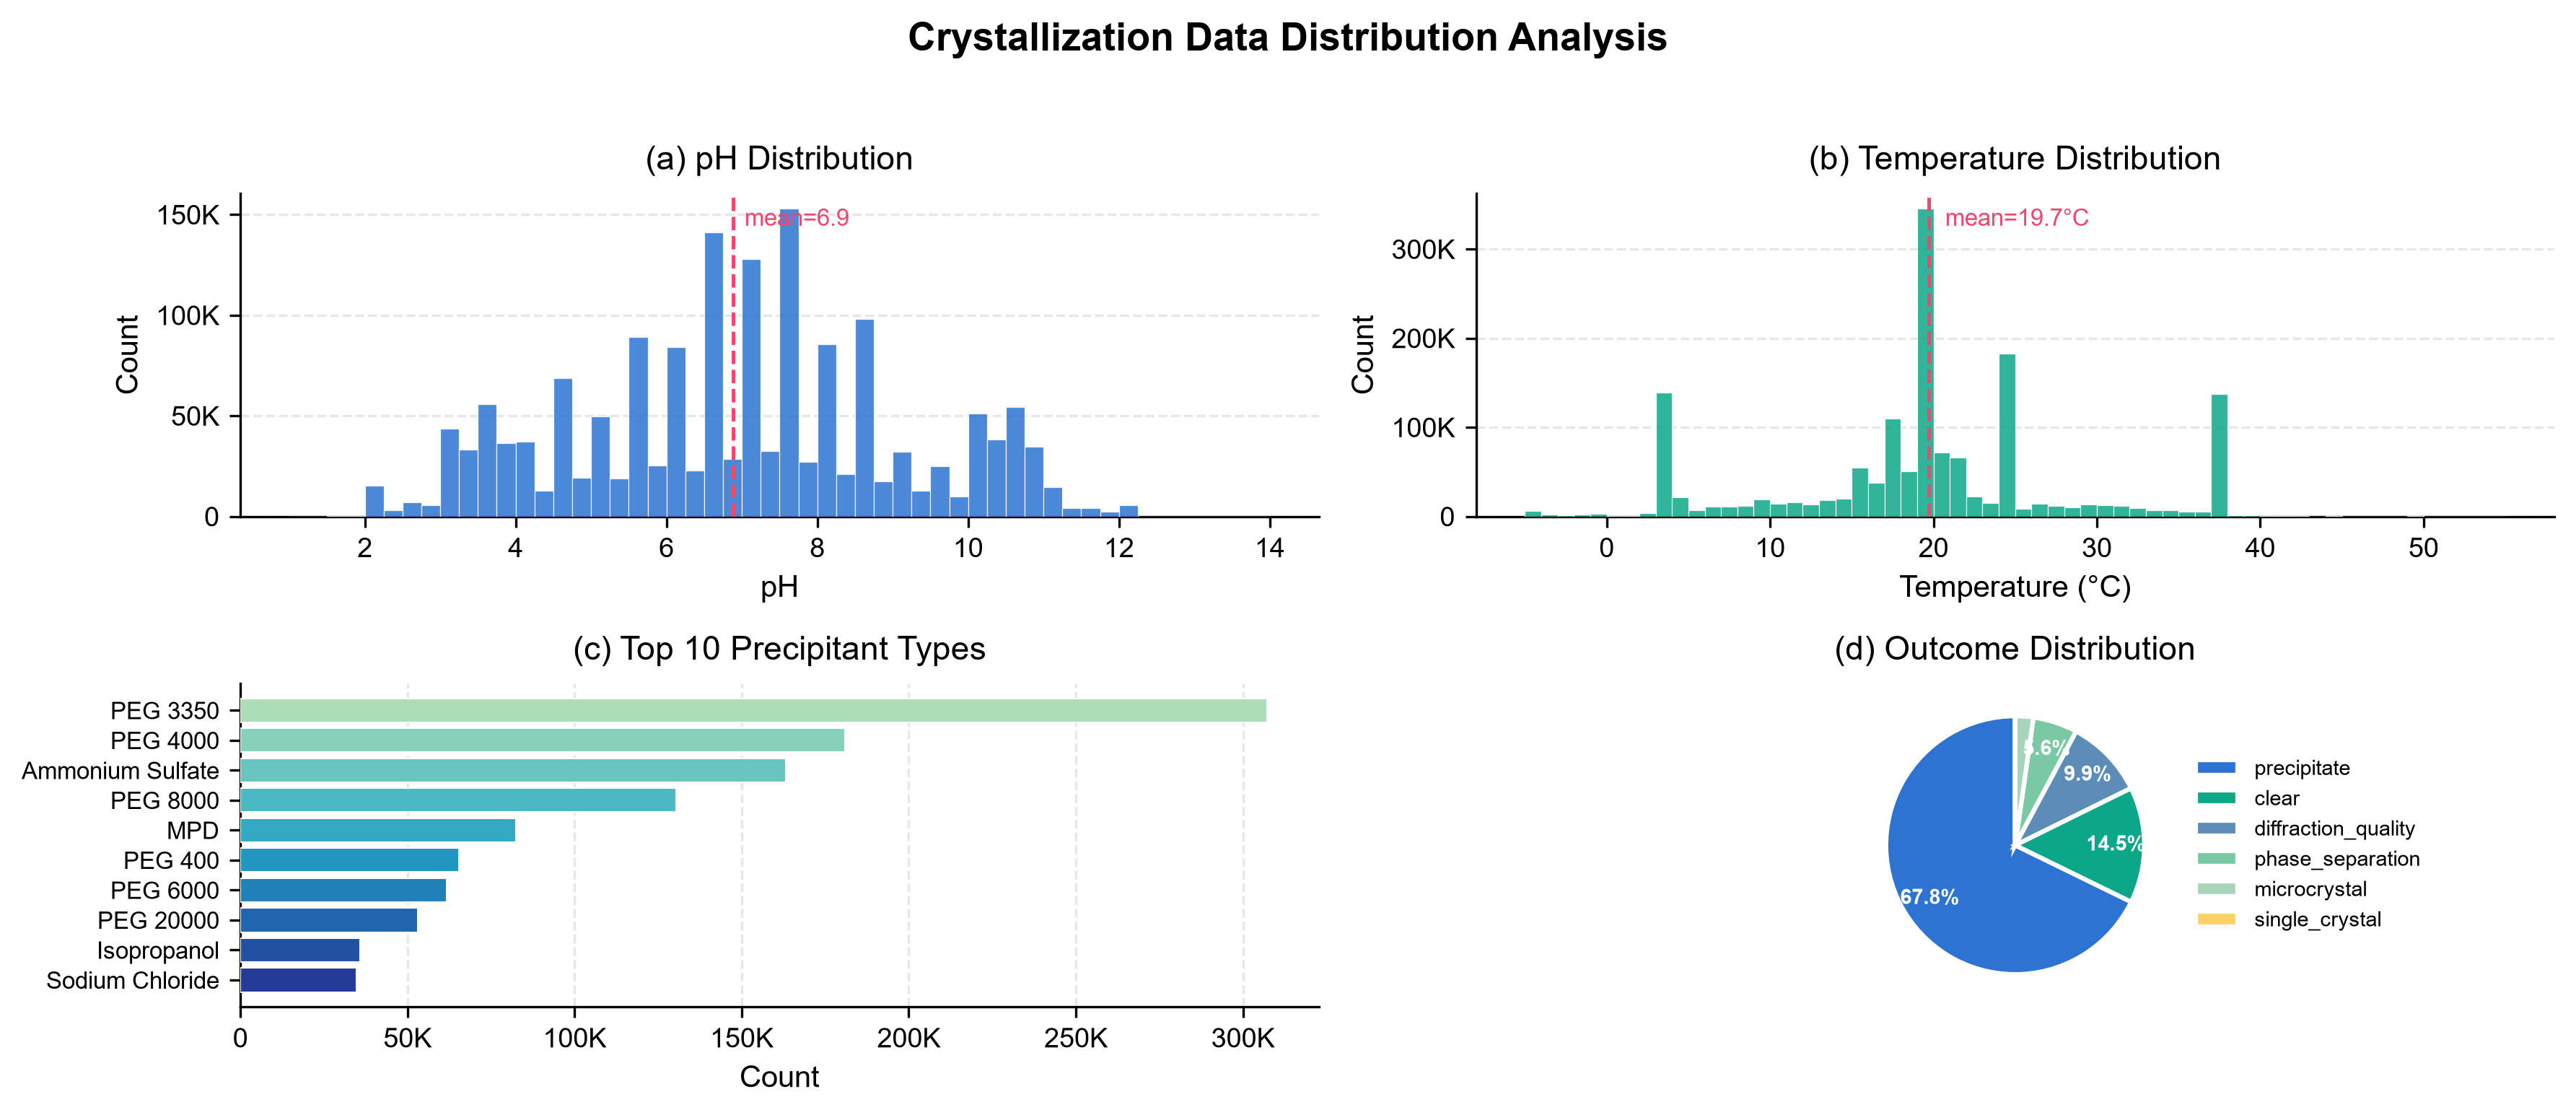
\includegraphics[width=\textwidth]{figures/fig8_distribution_analysis.png}
\caption{\textbf{Distribution analysis.} (a)~Outcome balance: success 18.8\% vs.\ failure 81.2\%, with experimental/synthetic breakdown. (b)~Data source composition: 20.1\% experimental, 79.9\% synthetic. (c)~Key metrics summary.}
\label{fig:distanalysis}
\end{figure}

% ═══════════════════════════════════════════════════════
% REFERENCES
% ═══════════════════════════════════════════════════════
\clearpage
\begin{thebibliography}{16}

\bibitem{mcpherson2014}
McPherson, A. \& Gavira, J.\,A.
Introduction to protein crystallization.
\textit{Acta Crystallogr.\ F} \textbf{70}, 2--20 (2014).

\bibitem{chayen2008}
Chayen, N.\,E. \& Saridakis, E.
Protein crystallization: from purified protein to diffraction-quality crystal.
\textit{Nat.\ Methods} \textbf{5}, 147--153 (2008).

\bibitem{berman2000}
Berman, H.\,M. \textit{et~al.}
The Protein Data Bank.
\textit{Nucleic Acids Res.} \textbf{28}, 235--242 (2000).

\bibitem{newman2005}
Newman, J. \textit{et~al.}
Towards rationalization of crystallization screening for small- to medium-sized academic laboratories.
\textit{Acta Crystallogr.\ D} \textbf{61}, 1426--1431 (2005).

\bibitem{rupp2009}
Rupp, B.
\textit{Biomolecular Crystallography: Principles, Practice, and Application to Structural Biology} (Garland Science, 2009).

\bibitem{overton2006}
Overton, I.\,M. \& Barton, G.\,J.
A normalised scale for structural genomics target ranking: the OB-Score.
\textit{FEBS Lett.} \textbf{580}, 4005--4009 (2006).

\bibitem{berman2009psi}
Berman, H.\,M. \textit{et~al.}
The Protein Structure Initiative Structural Genomics Knowledgebase.
\textit{Nucleic Acids Res.} \textbf{37}, D365--D368 (2009).

\bibitem{grazulis2012}
Gra\v{z}ulis, S. \textit{et~al.}
Crystallography Open Database.
\textit{Nucleic Acids Res.} \textbf{40}, D471--D477 (2012).

\bibitem{zdrazil2024}
Zdrazil, B. \textit{et~al.}
The ChEMBL Database in 2023.
\textit{Nucleic Acids Res.} \textbf{52}, D1180--D1192 (2024).

\bibitem{gilson2016}
Gilson, M.\,K. \textit{et~al.}
BindingDB in 2015.
\textit{Nucleic Acids Res.} \textbf{44}, D1045--D1053 (2016).

\bibitem{dana2019}
Dana, J.\,M. \textit{et~al.}
SIFTS: updated Structure Integration with Function, Taxonomy and Sequences resource.
\textit{Nucleic Acids Res.} \textbf{47}, D482--D489 (2019).

\bibitem{lin2023}
Lin, Z. \textit{et~al.}
Evolutionary-scale prediction of atomic-level protein structure with a language model.
\textit{Science} \textbf{379}, 1123--1130 (2023).

\bibitem{jancarik1991}
Jancarik, J. \& Kim, S.\,H.
Sparse matrix sampling: a screening method for crystallization of proteins.
\textit{J.\ Appl.\ Crystallogr.} \textbf{24}, 409--411 (1991).

\bibitem{luft2003}
Luft, J.\,R. \textit{et~al.}
A deliberate approach to screening for initial crystallization conditions of biological macromolecules.
\textit{J.\ Struct.\ Biol.} \textbf{142}, 170--179 (2003).

\bibitem{iso25012}
ISO/IEC 25012:2008.
Software engineering---Software product Quality Requirements and Evaluation (SQuaRE)---Data quality model.
International Organization for Standardization (2008).

\bibitem{wilkinson2016}
Wilkinson, M.\,D. \textit{et~al.}
The FAIR Guiding Principles for scientific data management and stewardship.
\textit{Sci.\ Data} \textbf{3}, 160018 (2016).

\end{thebibliography}

\end{document}
